\section{Bike Lanes Dataset}
To enrich our station and trip insights, we incorporate New York City's bike-route network, retrieved from the \href{https://data.cityofnewyork.us/dataset/New-York-City-Bike-Routes/}{NYC OpenData portal}.

\subsection{Dataset Structure}
Distributed as a single CSV file, the dataset provides a current snapshot of the bike network alongside a historical record, with the NYC Department of Transportation updating the file on an annual basis.

\subsubsection{Original Structure}
Each record answers four questions about one piece of the network: where it runs, what kind of facility it is, when it existed, and which route it belongs to.
\begin{itemize}
    \item \textbf{Geometry}: the set of lines defined in coordinates tracing the bike route.
    \item \textbf{Street}, \textbf{From Street}, \textbf{To Street}: the street the facility runs along.
    \item \textbf{Borough}: which of the five boroughs the segment lies in.
    \item \textbf{Facility Class}: the type of facility across four classes: \emph{Protected}, \emph{Conventional}, \emph{Shared Lane or Signed Route}, and \emph{Link}.
    \item \textbf{Status}: whether the facility is still in service or has been retired.
    \item \textbf{Installation Date} and \textbf{Retirement Date}: when the facility opened and, for facilities no longer in service, when it was removed.
    \item \textbf{Route ID}: the named route the segment forms part of.
    \item \textbf{Segment ID}: which piece of street the record covers. The numbering comes from LION (\emph{Linear Integrated Ordered Network}), the city's official street map, so every facility is pinned to a known piece of road.
\end{itemize}
Although finer classifications are recorded for each facility, they are excluded during ingestion.
Because these sub-types aggregate naturally into four primary classes, omitting them preserves structural simplicity without loss of informational value.

\subsection{Analysis and Insights}
The analysis addresses the two questions the dashboard puts to this dataset: what the network looks like today, and how it got there.

\paragraph{The Network Today}
Figure~\ref{fig:bike_lanes_map} draws every segment in service, coloured by facility class.
The lanes alone redraw the city, which is what makes this layer usable as a spatial backdrop, but the colour carries the actual finding: protection is not distributed evenly.
Manhattan is the only borough where \emph{Protected} is the majority class, at $54\%$ of its segments, while Brooklyn sits at $26\%$ and leans on \emph{Conventional} striping instead.
Brooklyn, Queens and Staten Island each leave roughly a quarter of their network as \emph{Shared Lane or Signed Route}, which amounts to a marking and a sign rather than a facility.
A rider crossing a borough line can therefore drop a protection level without leaving the network, and surfacing that contrast is precisely why the map is coloured this way rather than uniformly.

\begin{figure}[H]
    \centering
    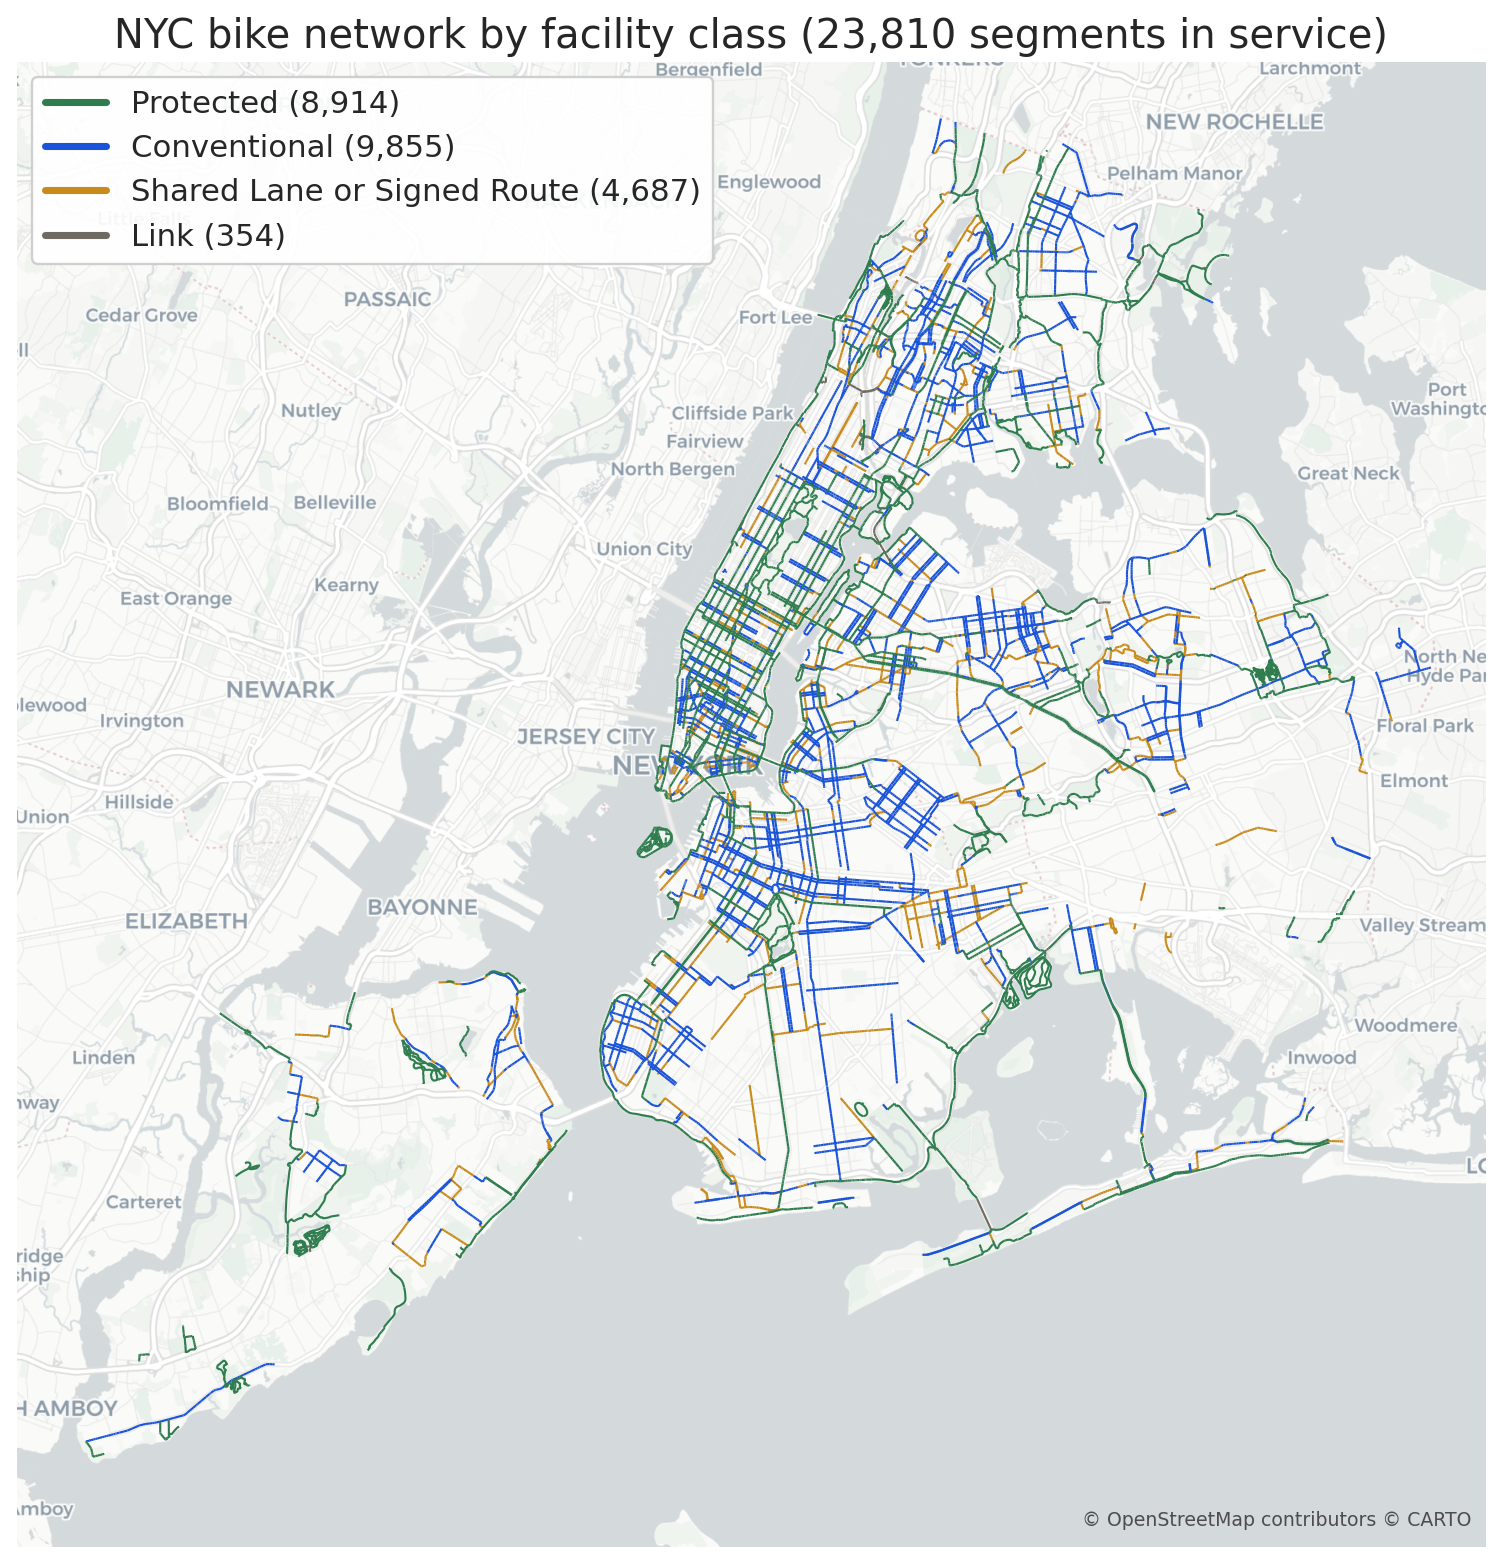
\includegraphics[width=.86\textwidth]{../media/bike_lanes_map.png}
    \caption{The bike-route network in service, coloured by facility class over the same palette and basemap the dashboard uses. Counts in the legend are segments, not kilometres.}
    \label{fig:bike_lanes_map}
\end{figure}

\paragraph{How the Network Grew}
Because retired facilities are kept, the network can be replayed year by year.
Figure~\ref{fig:bike_lanes_history} counts installations above the axis and retirements below it, the same form the dashboard uses to let the user step back through the network's history.
The build-out is overwhelmingly recent: $21{,}207$ of the $28{,}983$ records date from 2007 onward, whereas the $2{,}893$ predating 1996 are mostly protected off-street infrastructure, greenways, park drives and bridge crossings absorbed into the network rather than built as bike lanes.

The bars below the axis need to be read carefully, and this is the more interesting result.
Two thirds of all retirements ($66.9\%$) are matched by a new record on the same stretch of street installed the very same day, and $71\%$ of those come back \emph{better} protected, most commonly a conventional lane rebuilt as a protected one.
The red bars therefore measure churn from the upgrade programme far more than they measure lanes being taken away, a reading the data dictionary itself supports when it warns that ``retired bicycle facilities do not inherently indicate the removal of a bicycle facility''.

\begin{figure}[H]
    \centering
    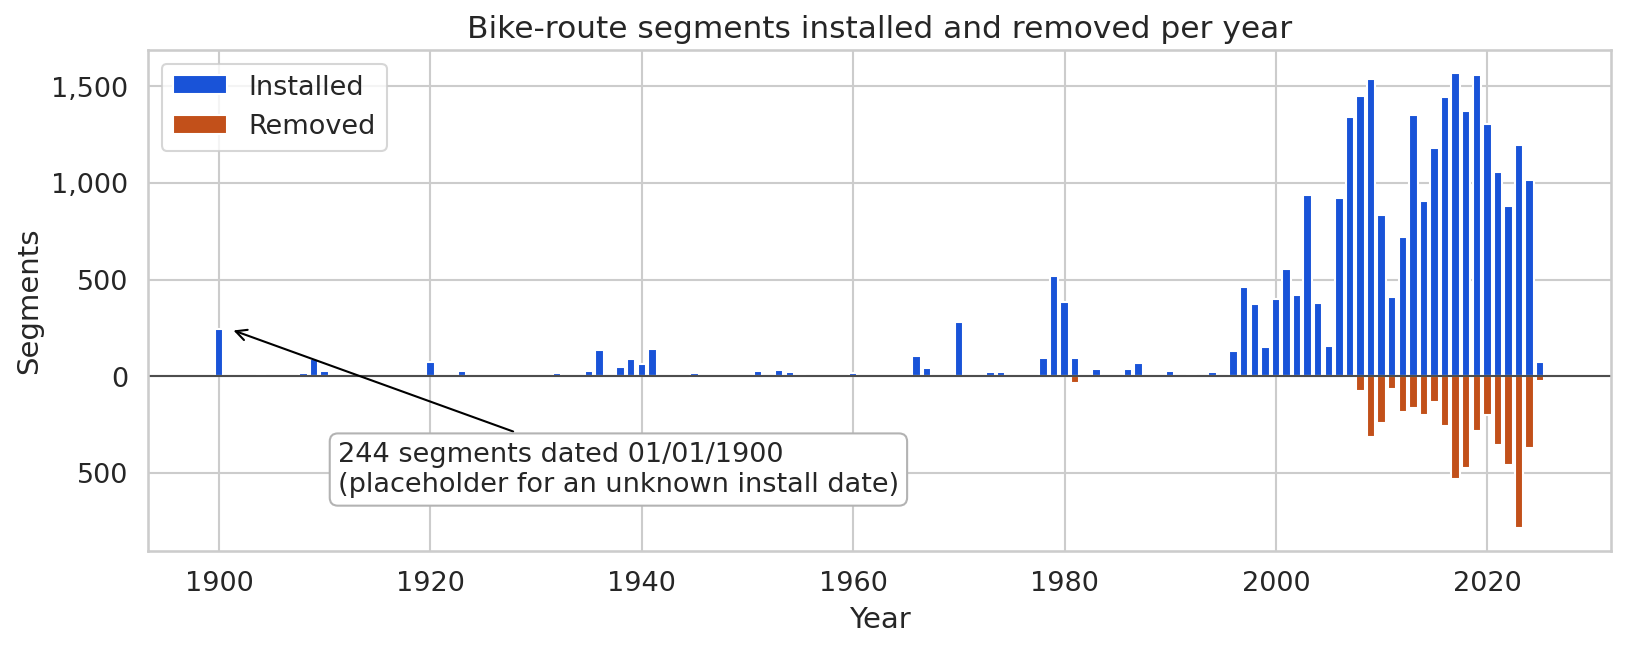
\includegraphics[width=\textwidth]{../media/bike_lanes_history.png}
    \caption{Segments installed and removed per year. Bars below the axis are retirements, two thirds of which are same-day rebuilds of the same stretch of street rather than removals.}
    \label{fig:bike_lanes_history}
\end{figure}

\subsection{Data Quality}
Every column we consume is fully populated, every geometry parses, and none falls outside New York.
The issues are therefore not gaps but mismatches between what fields are named and what they contain, all verified in the \href{https://github.com/davide-dona/nyc-bike-data-visualization/blob/main/src/notebooks/analysis.ipynb}{\underline{Jupyter notebook}} against the data dictionary.

\paragraph{Identifier Semantics}
Neither identifier is a row key, and treating either as one is the easiest mistake to make with this file.
The Segment ID names a stretch of street rather than a record, so it repeats every time that stretch is rebuilt: $4{,}603$ values carry more than one record, covering $9{,}489$ of the $28{,}983$ rows.
The Route ID names a route and is shared along its whole length, with a median of three segments and up to $158$, which is what lets the dashboard highlight an entire corridor from a single hovered segment.
The attribute that does link a facility to the one it superseded is among those dropped during preprocessing, so that lineage is unavailable downstream.
Our database keys rows on the segment, its installation date and its status together, a combination $155$ rows still collide on and which are discarded at load.

\paragraph{Sentinel Installation Dates}
The installation date is never null, which makes the file look complete under a missing-value check, but unknown dates are encoded as the placeholder \texttt{01/01/1900} rather than left blank; $244$ segments ($0.8\%$) carry it, $196$ of them still in service.
Because that sentinel is the earliest date in the file, and the year slider derives its lower bound from the earliest installation date, a single placeholder stretches the control across $126$ years of which only $67$ contain anything.

\paragraph{Status Contradicting the Dates}
The data dictionary fixes the invariant tying the two together: a current facility carries no retirement date, and a retired one always does.
Three records break it, all retired segments on 9th Avenue in Manhattan with no retirement date.
As noted in the Dataset Structure section, status never leaves the database, so our year filter is written on the dates alone; these three therefore survive into the present-day network instead of being filtered out with the rest of the retired infrastructure.
One further record, on Borinquen Place, is retired two years before its own installation date.
The volumes are small enough not to distort the map, but they are the reason the filter cannot be tightened to treat status and the dates as interchangeable.

\paragraph{Class Is a Maximum, Not a Description}
Facility class reports ``the HIGHEST facility class found along a segment'', so a street with a protected lane on one side and a shared lane on the other is drawn purely as protected.
This affects $720$ segments ($2.5\%$), which is small enough to leave the map's colouring unchanged but means it should be read as the best facility available on a segment rather than the facility on both sides of it.
